\documentclass{standalone}
\usepackage{tikz}
\begin{document}

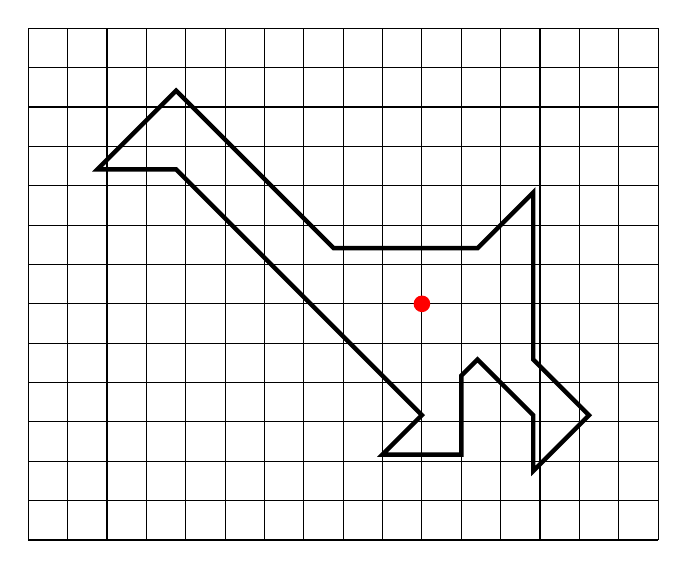
\begin{tikzpicture}
\draw[step=5mm] (-5.0, -3.0) grid (3.0, 3.5);
\draw[ultra thick]
    ({-1-3/2*sqrt(2)}, {2+1/2*sqrt(2)}) --
    ({1-3/2*sqrt(2)}, {1/2*sqrt(2)}) --
    ({1/2*sqrt(2)}, {1/2*sqrt(2)}) --
    ({sqrt(2)}, {sqrt(2)}) --
    ({sqrt(2)}, {-1/2*sqrt(2)}) --
    ({3/2*sqrt(2)}, {-sqrt(2)}) --
    ({sqrt(2)}, {-3/2*sqrt(2)}) --
    ({sqrt(2)}, {-sqrt(2)}) --
    ({1/2*sqrt(2)}, {-1/2*sqrt(2)}) --
    ({1/2}, {1/2-sqrt(2)}) --
    ({1/2}, {-1/2-sqrt(2)}) --
    ({-1/2}, {-1/2-sqrt(2)}) --
    ({0}, {-sqrt(2)}) --
    ({-1-3/2*sqrt(2)}, {1+1/2*sqrt(2)}) --
    ({-2-3/2*sqrt(2)}, {1+1/2*sqrt(2)}) -- cycle;
\fill[red] (0,0) circle (3pt);
\end{tikzpicture}

\end{document}